%% ProcessMusic.tex
%% V0.1
%% 2012/10/23
%% by Kyle Kastner
%%
%% requires IEEEtran.cls version 1.7 or later
%% This file based on content from http://www.ctan.org/tex-archive/macros/latex/contrib/IEEEtran/

\documentclass[journal]{IEEEtran}
\usepackage[labelfont=bf]{caption}
\captionsetup[figure]{labelformat=parens}
\usepackage{graphicx}
\usepackage{amsmath}
\usepackage{flushend}
\newcommand\numberthis{\addtocounter{equation}{1}\tag{\theequation}}
\begin{document}
\title{A Comparison of Quantization Methods}

\author{Kyle Kastner and Johanna Hansen}%

\markboth{Project 2: Quantization}{}
\maketitle

\begin{abstract}
Quantization is an important technique in modern communication and data systems. Linear, non-linear, and vector quantization
implementations have different characteristics and implementation concerns. Quantifying the differences in performance, and discussing 
the implementation issues associated with each technique, we show some of the trade offs made when choosing one of these quantization methods.
\end{abstract}
% IEEEtran.cls defaults to using nonbold math in the Abstract.
% This preserves the distinction between vectors and scalars. However,
% if the journal you are submitting to favors bold math in the abstract,
% then you can use LaTeX's standard command \boldmath at the very start
% of the abstract to achieve this. Many IEEE journals frown on math
% in the abstract anyway.

% Note that keywords are not normally used for peerreview papers.
\begin{IEEEkeywords}
Quantization, linear, vector, $\mu$-law, k-means.
\end{IEEEkeywords}

\IEEEpeerreviewmaketitle
\section{Introduction}
\IEEEPARstart{Q}{uantization} methods are crucial to modern technology. Quantization techniques have fueled 
advancements in communications, computing, and data processing. In this paper, we will compare linear and non-linear 
quantization methods at various bit levels, and discuss the complexities associated with each technique.

\subsection{Background}
Conveying information with minimal data has been and continues to be an important part of technology and research. Passwords, 
military codes, cellular communications, and compression are either in whole or in part based on this concept. One of the simplest ways
to achieve data reduction is to eliminate data that does not transmit useful information. This elimination, done correctly, can 
greatly reduce the amount of data required to transmit information, such as words in a conversation.

\subsection{Overview}
Several different methods of quantization will be shown and compared in the following pages. Implementations of linear, 
$\mu$-law, and vector quantizers were run against different audio files, generating results for mean squared error and 
signal to noise ratio. We also take special care to discuss the implementation details of each quantization type.

\subsection{Goal}
Our goal in this paper is to identify different ways to perform quantization, compare the performance of each method discussed, show 
implementation examples for each, and discuss the engineering trade-offs associated with choosing a particular quantization scheme.

\section{Error}
Quantization is considered a "lossy" scheme, which means that during the quantization operation, data is thrown out and cannot
be recovered. This data may or may not contain useful information about the signal being quantized. When data is lost, error is
introduced, known as quantization error. Given a sampled input $x_n$, quantization error can be shown as \cite{DSPBook}
\begin{equation}
    x_q = x_n + e_n
\end{equation}
where $e_n$ is the quantization error. Quantizer performance will be measured by comparing the error introduced by different methods
while holding system inputs and parameters fixed. Two basic measurements convey the amount of error introduced, Normalized Root Mean Squared Error (NRMSE)
and SNR (Signal To Noise Ratio).

\section{Linear Quantization}
\subsection{Formulation}
Linear quantization is the simplest method for applying quantization to a signal. The linear quantizer can be implemented as a sample
and hold operation in hardware, or by the integer division method available in most computer languages. For an input sample $x_n$, the
linear quantizer can be formulated as follows \cite{DSPBook}
\begin{equation}
    x_q = int(\frac{x_n*2^B}{x_{max} - x_{min}}) 
    \label{eq:linear}
\end{equation}
where $B$ is the number of quantization bits.

\subsection{Performance}
The linear quantizer has near-zero computational overhead, and with a relatively large number of quantization bits or a narrow 
dynamic range, quantization error can be fairly low. However, the linear quantizer is a poor choice for many systems, as there are
alternatives which introduce less quantization error for the same system parameters $x_{max}$, $x_{min}$, and $B$.

\subsection{Visualization}
\begin{figure}[h!]
\centering
  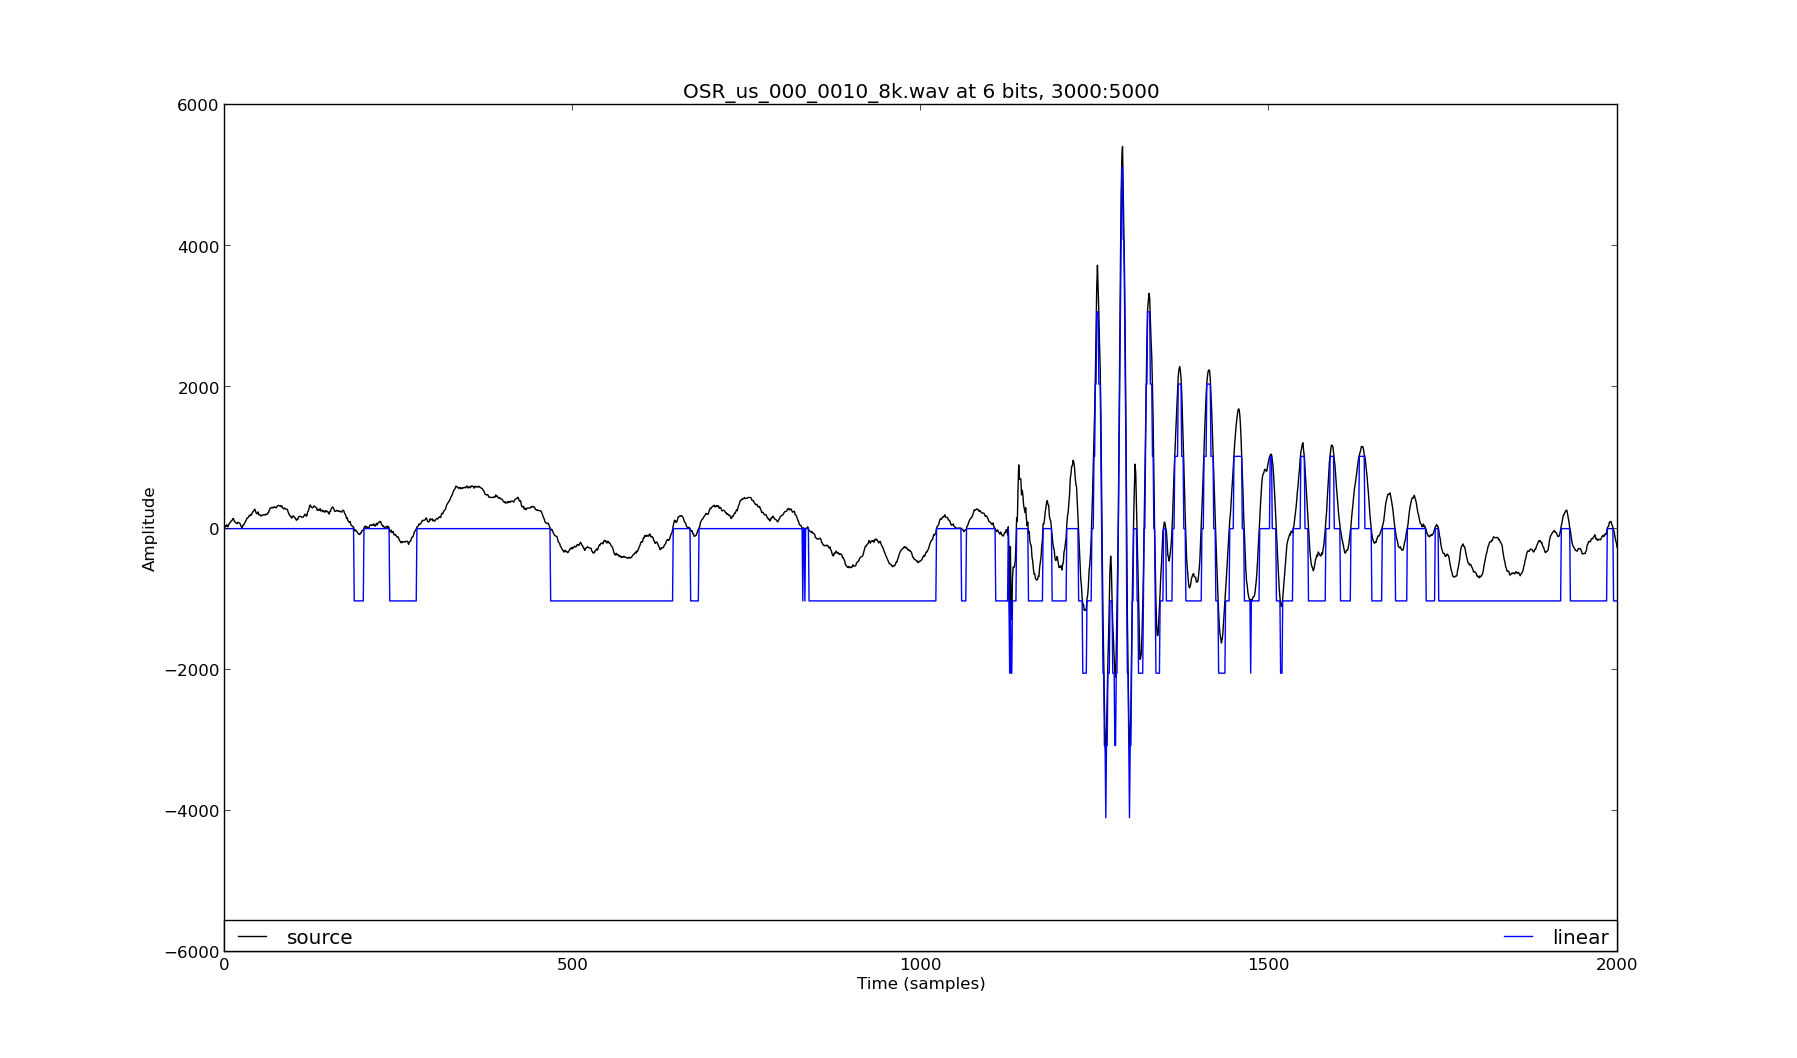
\includegraphics[width=0.45\textwidth]{linear_6bit.png}
\caption{Linear quantization, $B = 6$}
\label{fig:linear}
\end{figure}
The image in Figure \ref{fig:linear} shows an example of linear quantization, applied to an audio file containing speech. 

\section{Non-linear Quantization}
Non-linear quantization covers a wide variety of quantization techniques. One of the most common non-linear quantizers is based on the 
$\mu$-law algorithm, which uses logarithmic formulas to map input to a compressed domain (companding), apply a linear quantizer, then
invert the companding stage (expanding) in order to perform non-linear quantization. There are other methods of non-linear quantization that use
different algorithms, such as the $A$-law formula or specialized formulas for specific data types. 

\subsection{Formulation}
The companding stage of the $\mu$-law quantizer uses the following formula \cite{CiscoWeb}:
\begin{equation}
    x_q = \frac{ln(1 + \mu \lvert x_n \rvert)}{ln(1 + \mu)}sign(x_n), -1 \le x_n \le 1  
\end{equation}

Linear expansion as in Equation \ref{eq:linear} is applied, then an inversion formula is applied, where  
\begin{equation}
    y_n = \frac{1}{\mu}((1-\mu)^{\lvert y_q \rvert}-1), -1 \le y_q \le 1
\end{equation}
shows the inversion formula.

\subsection{Performance}
The $\mu$-law quantizer adds a minimal amount computational overhead, in exchange for superior error rates for commonly quantized data types
(music, speech, etc.). The $\mu$-law quantizer can be extended to an adaptive $\mu$-law quantizer, or combined with the $A$-law quantizer to
form a switching adaptive scheme.

\subsection{Visualization}
\begin{figure}[h!]
\centering
  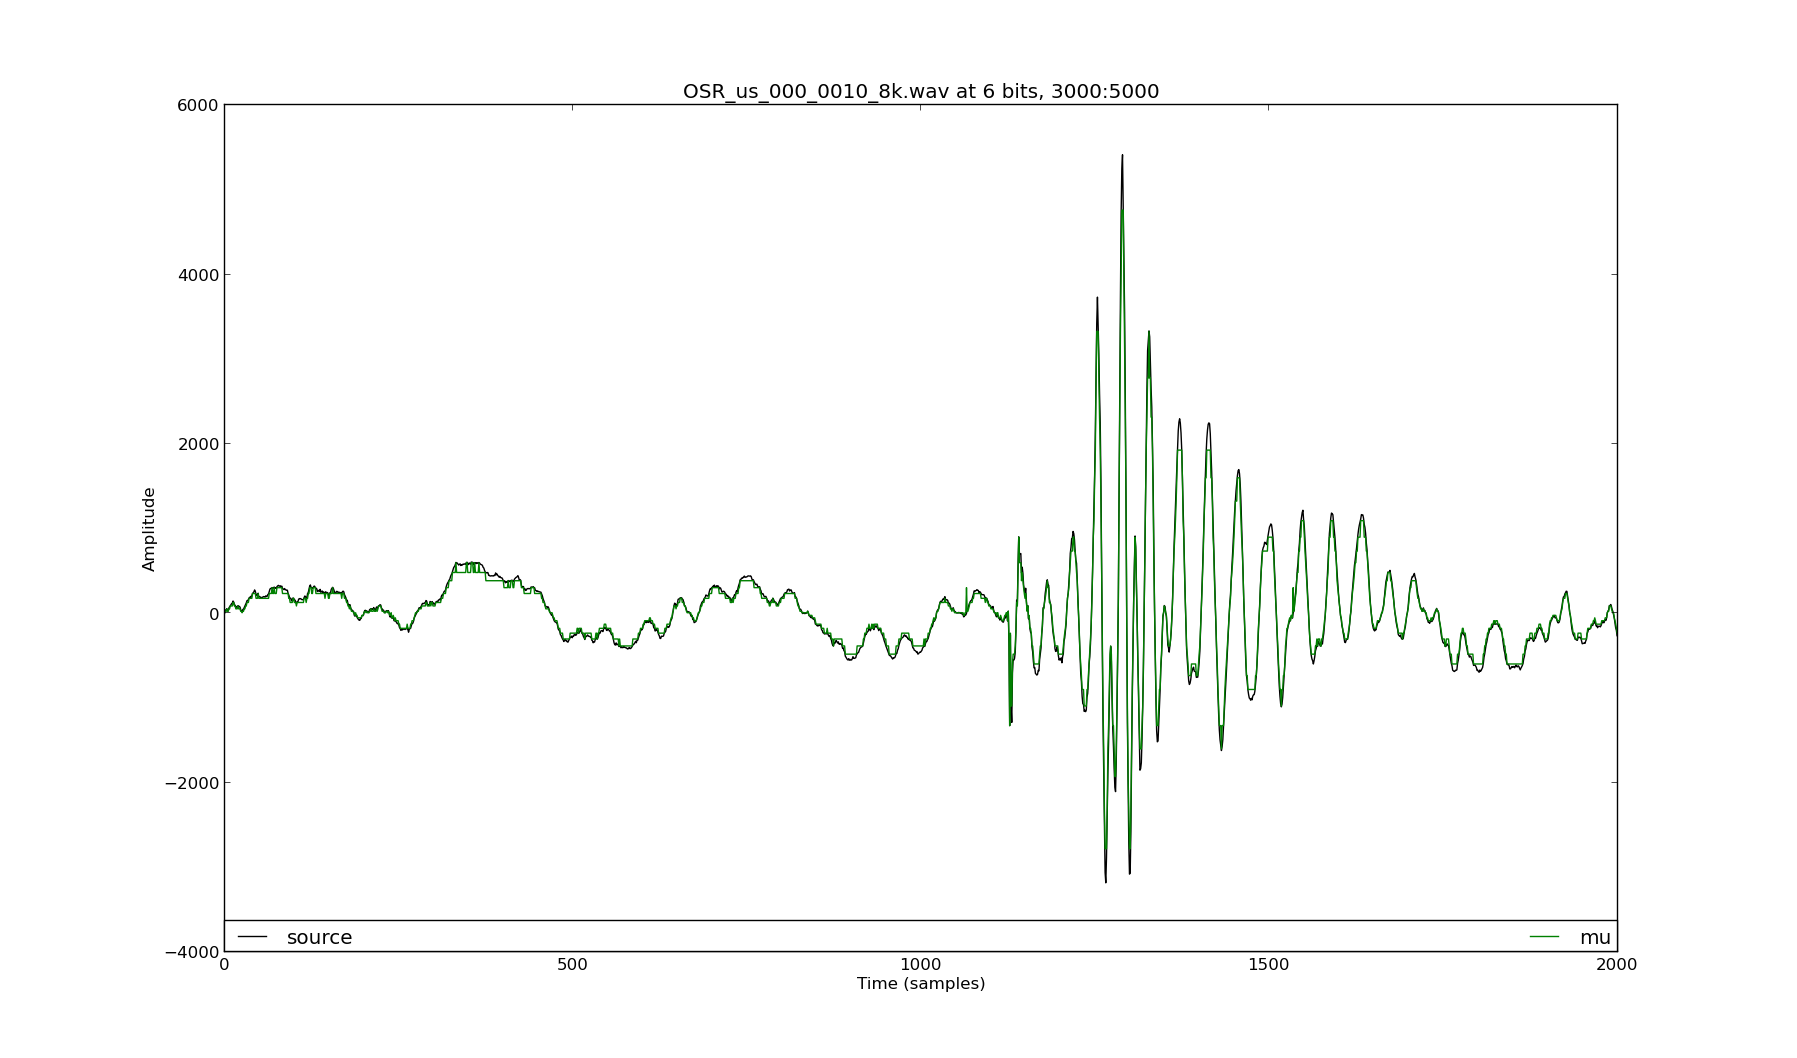
\includegraphics[width=0.45\textwidth]{mu_6bit.png}
\caption{$\mu$-law quantization, $B = 6$, $\mu = 255$}
\label{fig:mu}
\end{figure}

\section{Vector Quantization}
Vector quantization can be seen as a further extension of non-linear quantization. Rather than assigning boundaries based on a set formula, the 
vector quantizer uses k-means clustering of an example data set to intelligently set bit boundaries. There are many issues to be dealt with 
when implementing the k-means clustering section of the vector quantizer, which will be discussed in the sections below.

\subsection{K-means Initialization}
K-means clustering is a technique for associating a set of values with $k$ cluster centroids, where $k$ is a predefined integer. This works very well for 
quantization, as the value for $B$ is pre-determined, which means $k = 2^B$. To perform clustering, there are two primary stages: initialization, 
and association. K-means clustering is extremely sensitive to initialization, and there are several different ways to perform the initialization stage. 

\subsubsection{Value Initialization}
Value initialization is the simplest way to initialize k-means centroids.
\begin{equation}
    c_n = V, n = 1...k
\end{equation}
Examples for $V$ include $0$, the mean of the data set, the median of the data set, or the mode of the data set.

\subsection{Linear Initialization}
Linear initialization uses a similar approach to the linear quantizer, seen in Equation \ref{eq:linear}, to set centroid cluster values.
\begin{equation}
    c_n = x_{min} + \frac{n(x_{max} - x_{min})}{2^B}, n = 1...k 
\end{equation}

\subsection{Probabilistic Methods}
\subsubsection{Forgy Method}
The Forgy method for initialization takes $k$ samples at random from the data set, and uses those values to initialize the k-means centroids.
\begin{equation}
    c_n = \emph{X}, \emph{X} \in \{x_1...x_n\}, n = 1...k
\end{equation}

\subsubsection{Unknown Distribution Sampling}
The set of data to be quantized can be thought of as data with an unknown distribution. There are several techniques for sampling from unknown
distributions, including the rejection sampling and Metropolis-Hastings sampling techniques, which are the two techniques used for comparison in this
paper. The implementation of these two algorithms is outside the scope of this paper, but more information can be found in \cite{BayesianBook}.

\subsection{Sculptor's Method}
The Sculptor's method is a new method developed during work on this paper. While testing the different ways of initializing the k-means centroids, there
seemed to be large performance differences between the repeatable methods (Value, Linear) and the probabilistic techniques (Forgy, Rejection, 
Metropolis-Hastings). Unfortunately, probabilistic methods are difficult to test and quantify, due to the sensitivity of the k-means algorithm to
initialization. A repeatable method for initialization which provides performance approaching that of the probabilistic methods is desired. 
Method based on a center(s) of mass calculation were considered, but further exploration led to the creation of the 
Sculptor's method, formulated below.
\begin{equation}
    c_n = x_{min} + \frac{n(x_{max}-x_{min})}{2^B}\frac{\sum_{i=0}^{n}count(x_{min}+i)}{n}, n = 1...k 
\end{equation}
If one imagines the linear initialization method as a flat piece of clay, with lines evenly spaced across the length, then the placement of
centroids for the Sculptor's method can be found by compressing or expanding different sections of the clay. Compressing sections will decrease the
distances between lines, while stretching the clay will increase distance between lines. By thinking of the histogram of data as a "map" of pressure
applied to the clay, the distance between lines is inversely proportional to the summed count of values per bin (histogram area).

\subsection{Formulation}
Once initialization is completed through some method, the k-means algorithm iterates through each point in the data set, assigning each data point to a
centroid.
\begin{equation}
    x_c = min((x_q - c_n)^2), n = 1...k
\end{equation}
After a data point is assigned to a given centroid, the centroid value is updated.
\begin{equation}
    \forall x \in {x_c}, c_n = c_n(1-\alpha) + x\alpha, n = 1..k, 0 < \alpha < 1
\end{equation}
Here $x_c$ represents the set of values associated with each cluster by the previous assignment stage.
Once all data has been processed, each value associated with a cluster centroid is set to the value of that centroid. \cite{meansWeb}

\subsection{Performance}
Vector quantization has much more overhead than the previously discussed linear and non-linear techniques. Implementation is more complex, and 
there is a wide performance difference which depends on the initialization of k-means centroids. However, basing quantization levels on the content
of the data instead of an what the content is expected to be has some performance benefits, at the cost of introducing a large amount of delay in order
to keep the system causal.

\subsection{Visualization}
\begin{figure}[h!]
\centering
  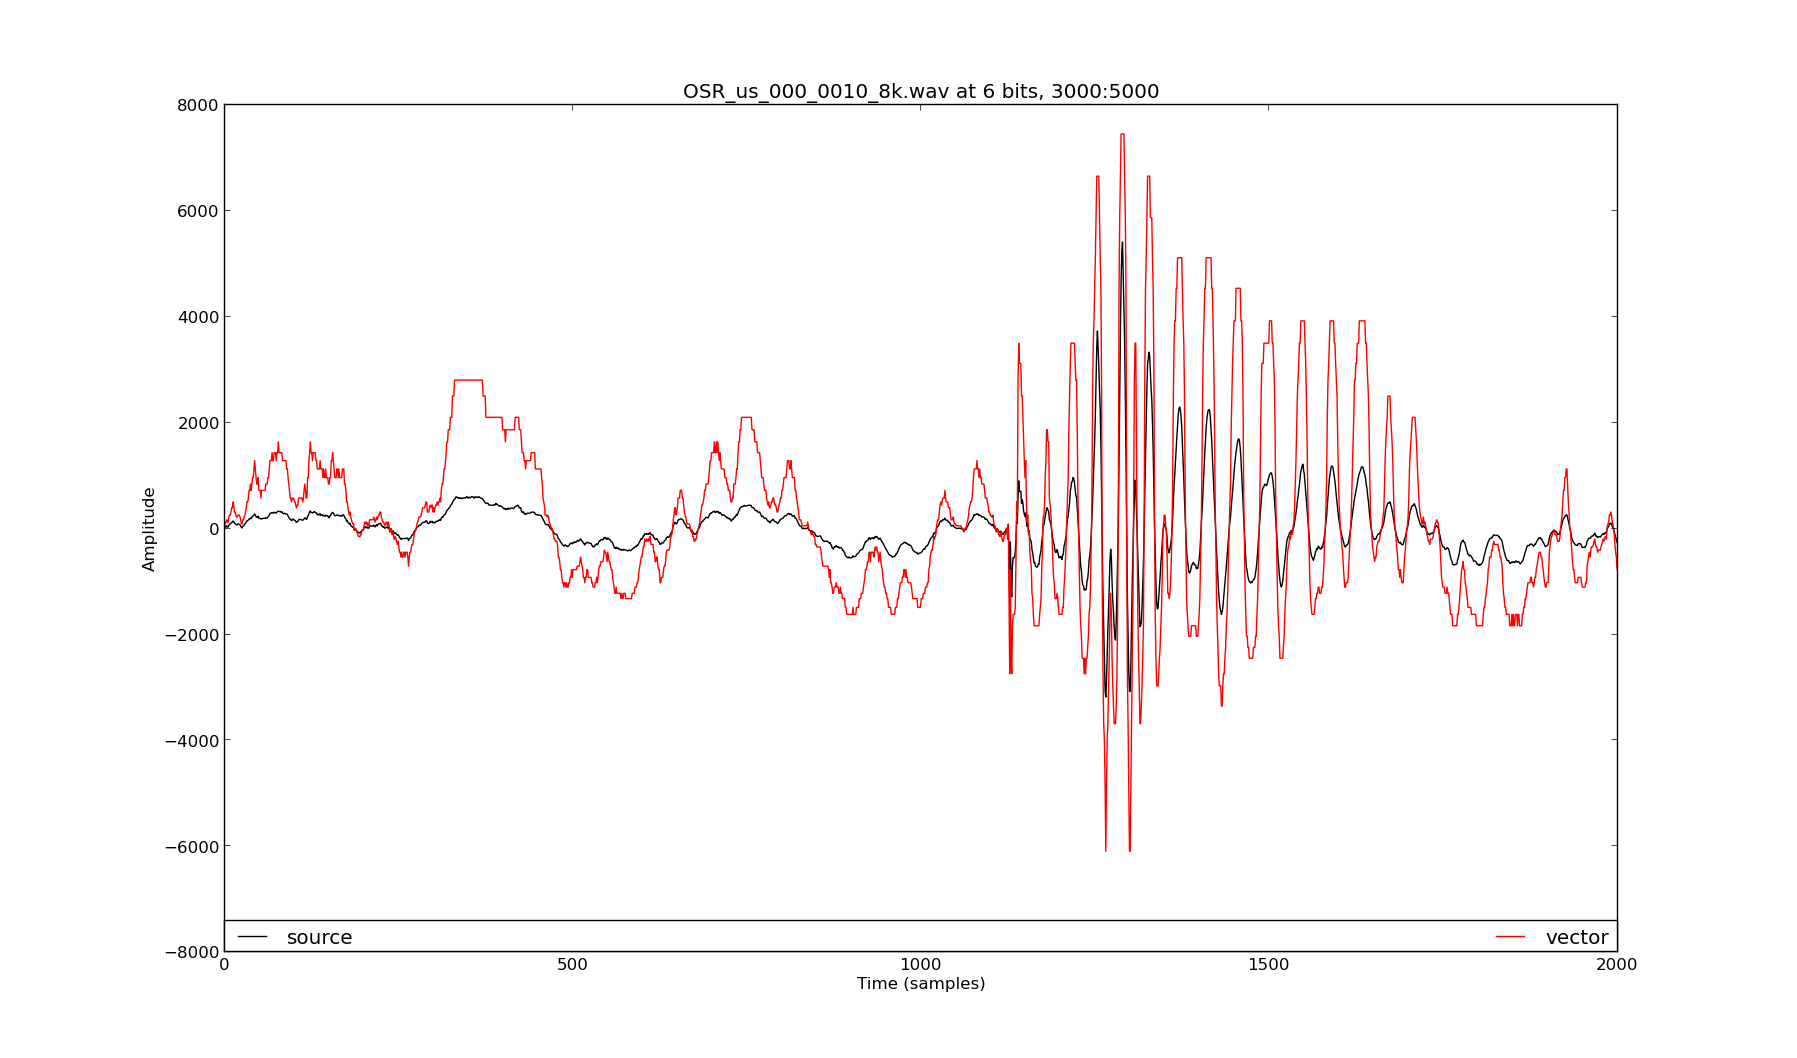
\includegraphics[width=0.45\textwidth]{vector_6bit.png}
\caption{Vector quantization, $B = 6$, $init = Sculptor's$}
\label{fig:vector}
\end{figure}

\section{Comparison}
The two measurements used to compare the various quantization schemes discussed above were Normalized Root Mean Squared Error (NRMSE), shown in Equation
\ref{eq:NRMSE}, and Signal to Noise Ratio (SNR), shown in Equation \ref{eq:SNR}. \cite{DSPBook}
\begin{equation}
    NRMSE = \frac{\sum_{i=0}^n (x_n - q_n)^2}{n}, n = length(x)
    \label{eq:NRMSE}
\end{equation}

\begin{equation}
    SNR = 10log(\frac{\sigma_x}{\sigma_q})
    \label{eq:SNR}
\end{equation}
The files used for this testing, as well as generation of Figures \ref{fig:linear},\ref{fig:mu},\ref{fig:vector}, were found at \cite{sourceWeb}. These
particular tests were run against the "OSR\_us\_000\_0010\_8k.wav" file, though other speech files from this site show similar results. Applying the
measurements to each of the quantization schemes, the following figures were generated. 
\begin{figure}[h!]
\centering
  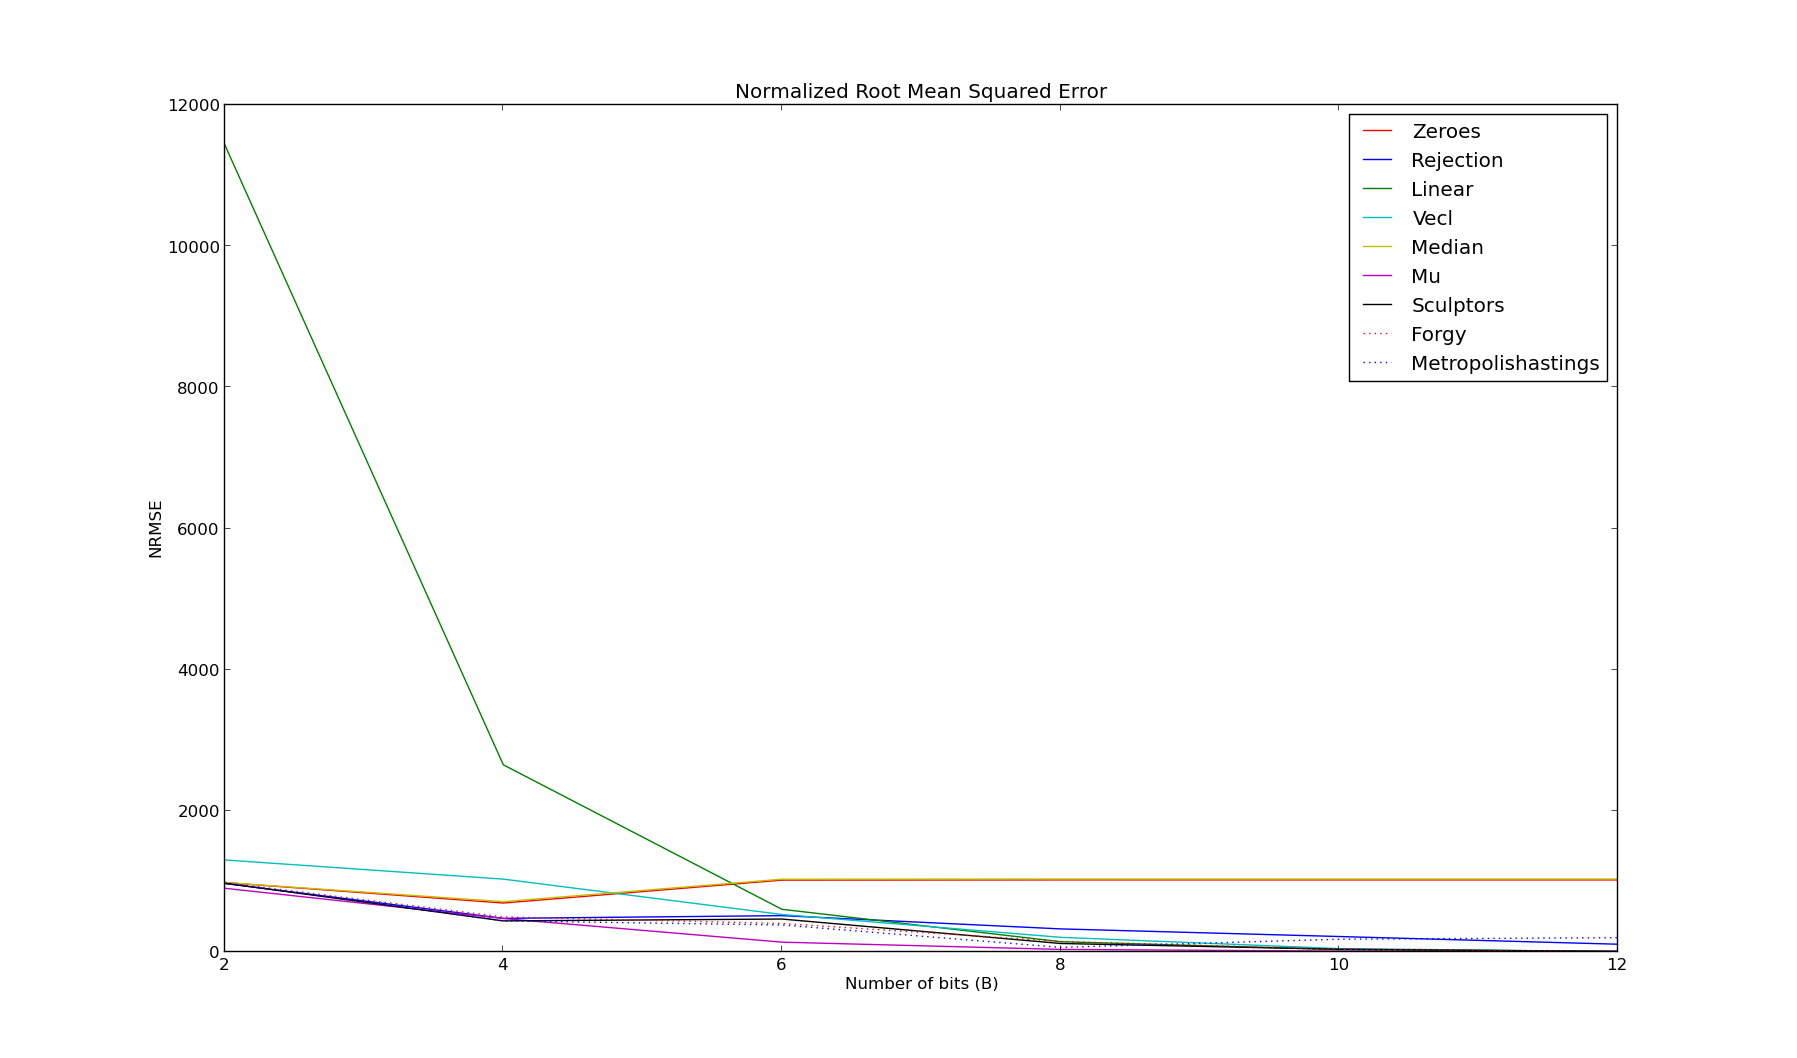
\includegraphics[width=0.45\textwidth]{NRMSE_all.png}
\caption{Normalized Root Mean Squared Error}
\label{fig:NRMSE_all}
\end{figure}
\begin{figure}[h!]
\centering
  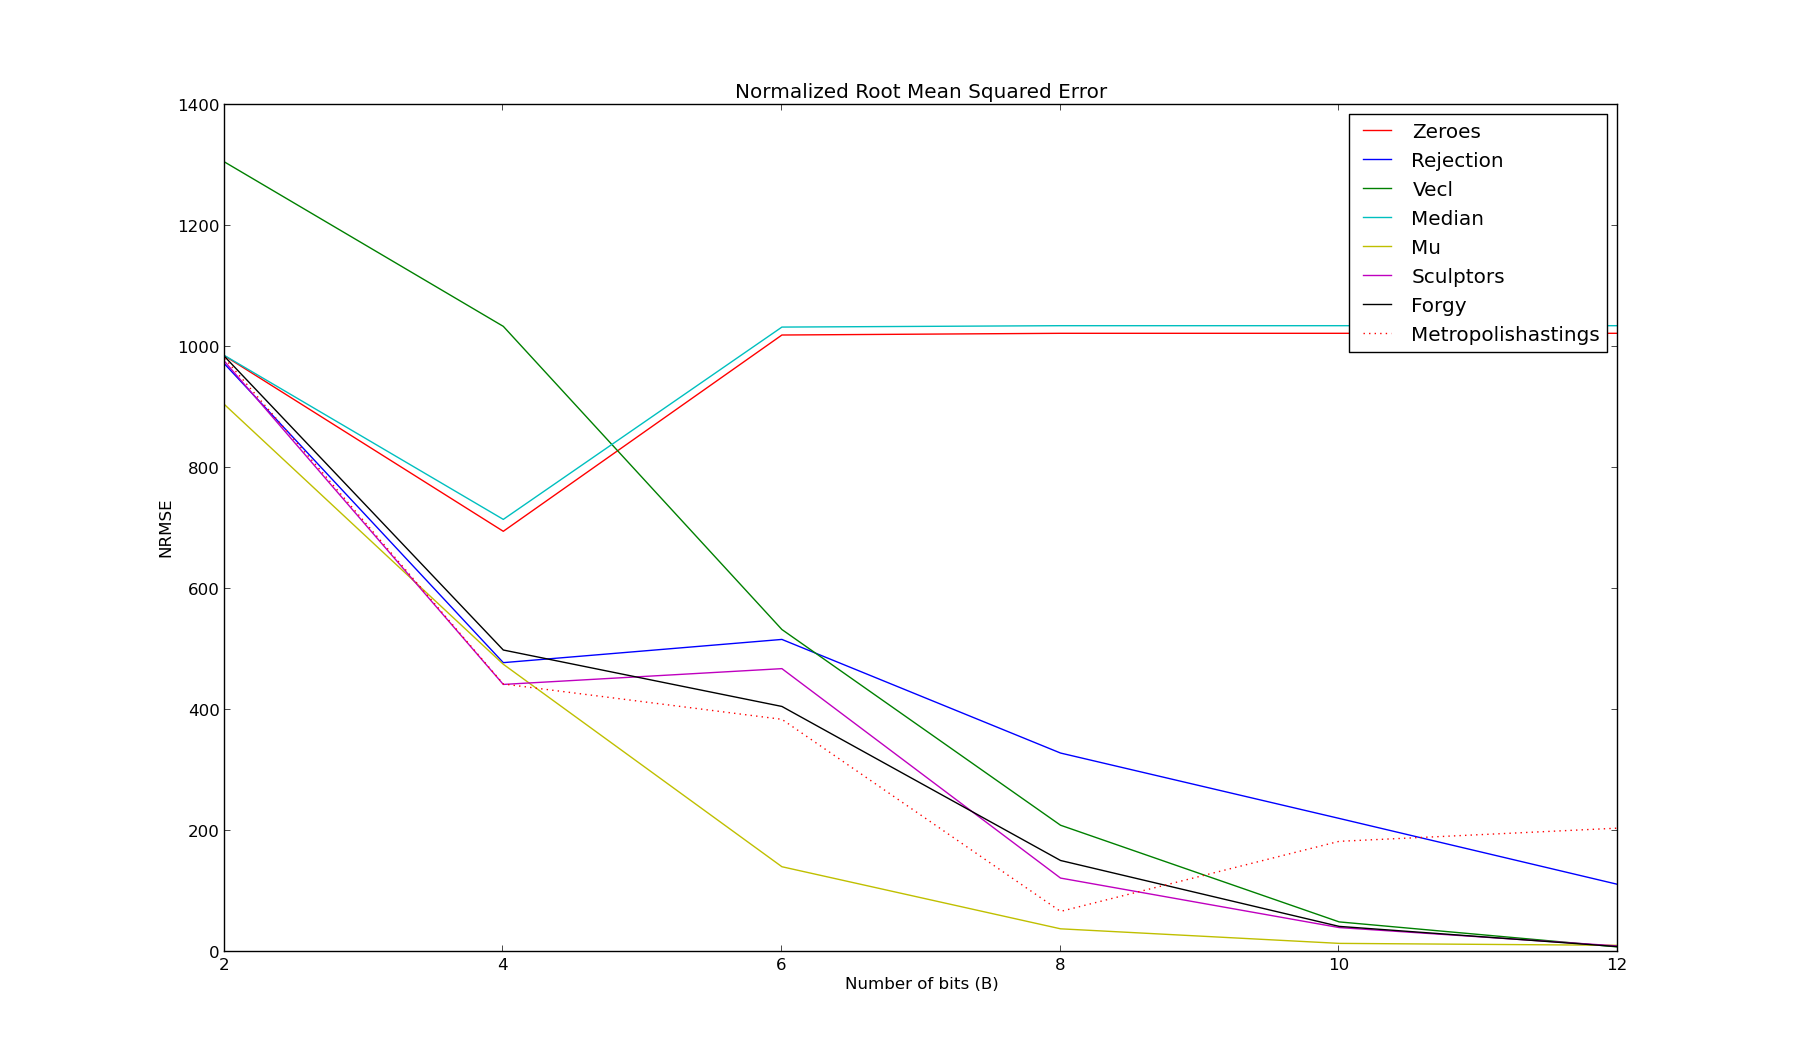
\includegraphics[width=0.45\textwidth]{NRMSE_nolinear.png}
\caption{Normalized Root Mean Squared Error, excluding linear quantization}
\label{fig:NRMSE_nolinear}
\end{figure}
\begin{figure}[h!]
\centering
  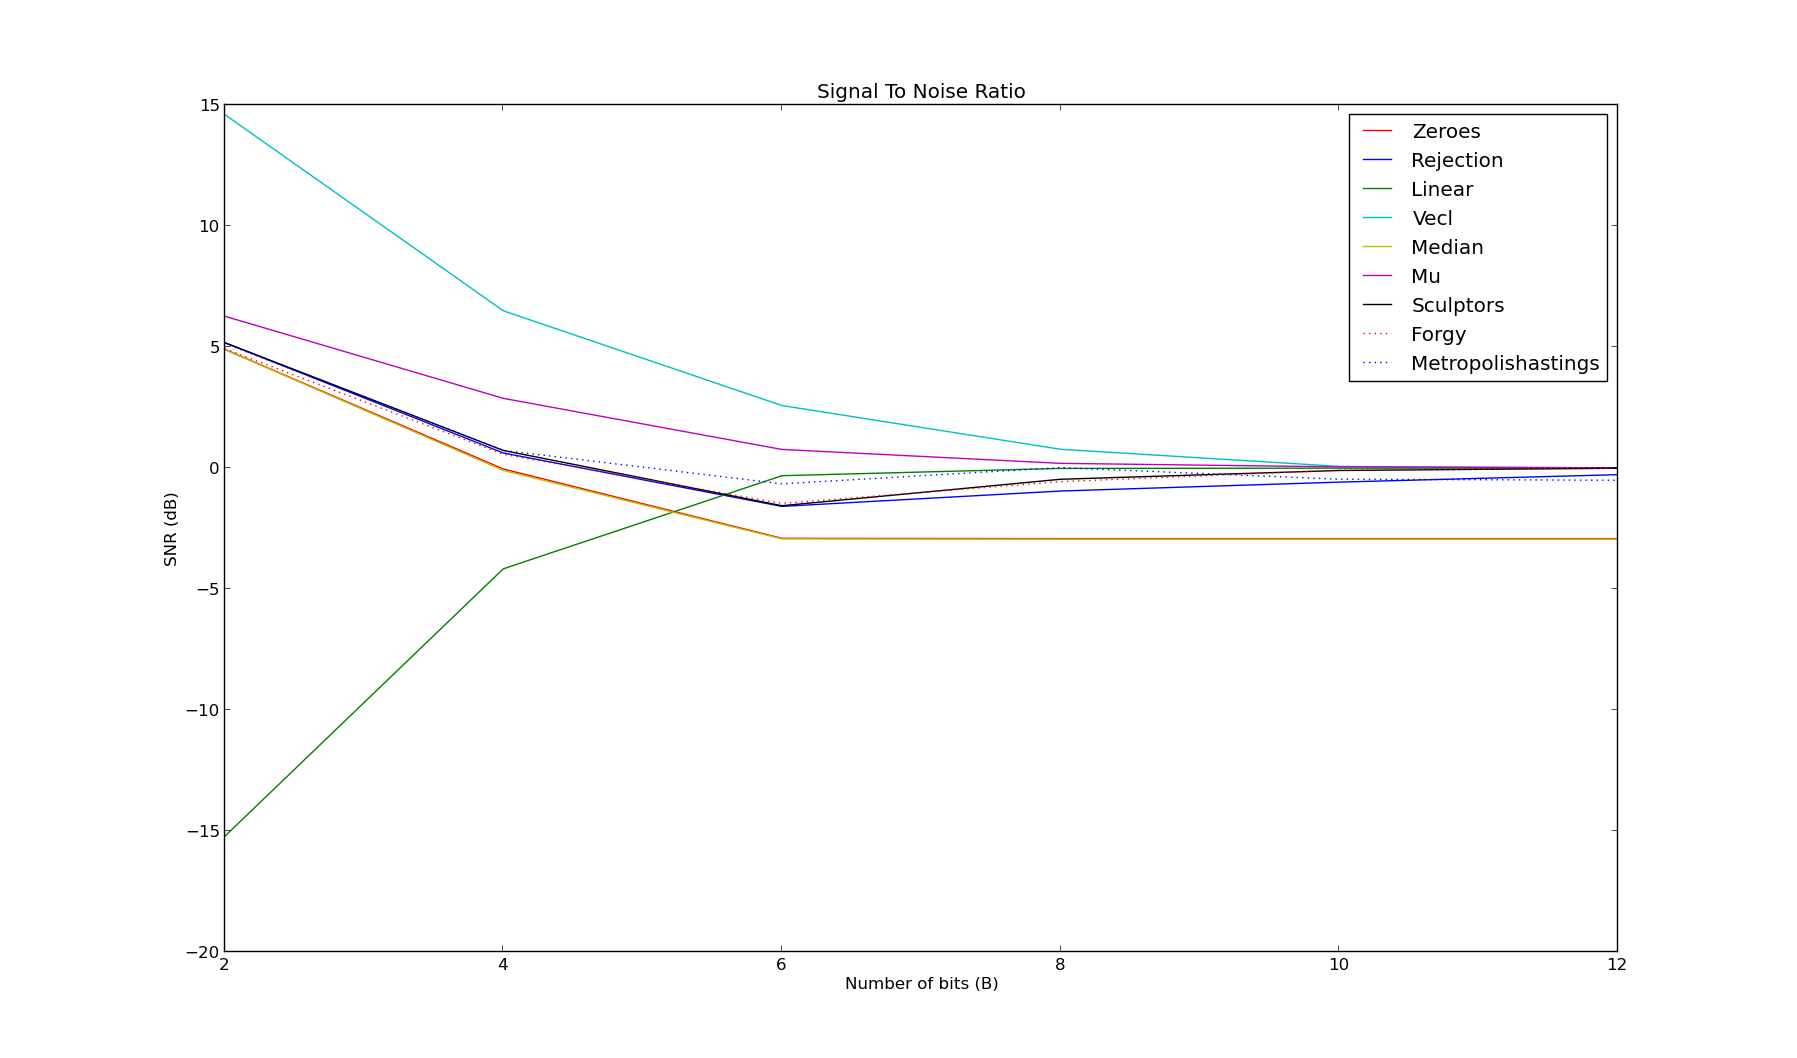
\includegraphics[width=0.45\textwidth]{SNR_all.png}
\caption{Signal To Noise Ratio}
\label{fig:SNR_all}
\end{figure}
\begin{figure}[h!]
\centering
  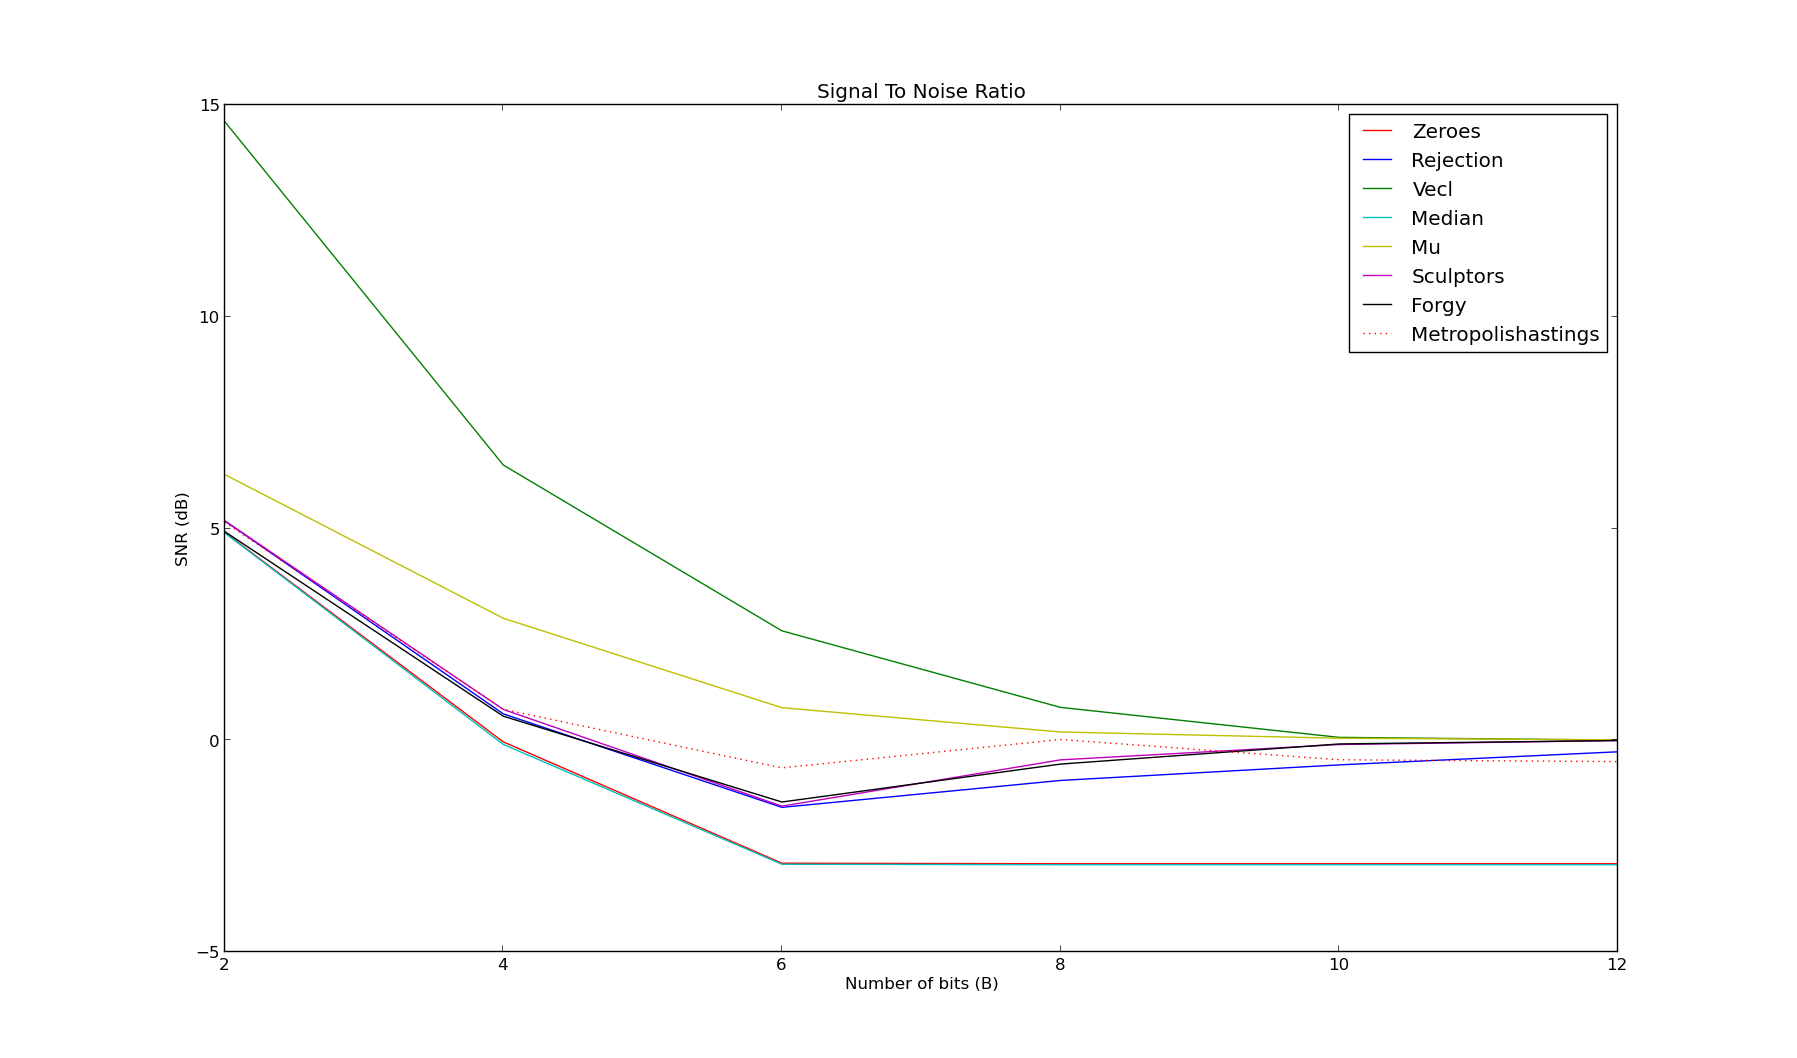
\includegraphics[width=0.45\textwidth]{SNR_nolinear.png}
\caption{Signal To Noise Ratio, excluding linear quantization}
\label{fig:SNR_nolinear}
\end{figure}

\section{Future Work}
More exploration and testing of the Sculptor's method is necessary. Testing against data sets besides speech data, as well as a larger sample set for
quantifying the performance of the probabilistic methods, will go a long way toward validating the results of this initial exploration. There is also 
room to test the Sculptor's method, without follow on k-means clustering, as a different method for non-linear quantization. Implementations of the 
$A$-law quantizer, and adaptive quantization schemes would add breadth to the test coverage, and allow for more accurate comparisons between the 
various methods.

\section{Conclusion}
This paper explored various algorithms for quantization. Using Normalized Root Mean Squared Error and Signal to Noise ratio measurements, 
linear, non-linear, and vector quantizers were compared for English speech data. A new type of initialization for vector quantizers, named
the Sculptor's method, was introduced. This method offers repeatable output, simplicity, and performance, and seems to compare favourably with 
existing techniques for vector quantization initialization. Readers of this paper should find the information here helpful in determining which
quantization methods are most appropriate for a given system.

\begin{thebibliography}{1}
\bibitem{DSPBook}
A. Oppenheim, R. Schafer, and J. Buck, \emph{Discrete Time Signal Processing}, 2nd Edition. Prentice-Hall, 1999.

\bibitem{CiscoWeb}
Cisco, \emph{Waveform Coding Techniques}. Retrieved November, 2012. http://www.cisco.com/en/US/tech/tk1077/technologies\_tech\_note09186a00801149b3.shtml 

\bibitem{BayesianBook}
A. Gelman, J. Carlin, H. Stern, D. Rubin, \emph{Bayesian Data Analysis}, 2nd Edition. CRC Press, 2004.

\bibitem{meansWeb}
S. Lloyd, "Least squares quantization in PCM", \emph{IEEE Transactions on Information Theory}. Volume 28, Issue 2, 1982.

\bibitem{sourceWeb}
"OSR\_us\_000\_0010\_8k.wav", \emph{Open Speech Repository}, American English. Telchemy Incorporated, Retrieved November, 2012.  
http://www.voiptroubleshooter.com/open\_speech/american.html 
\end{thebibliography}

% if you will not have a photo at all:
%\begin{IEEEbiographynophoto}{Kyle Kastner}
%Kyle is a graduate of Texas State University, B.S.E.E., who is currently pursuing an M.S.E.E at University of Texas-San Antonio.
%Research areas include powerline communications, cognitive radio, music classification and radiolocation techniques.
%He is curently employed by Southwest Research Institute, Division 16. 
%\end{IEEEbiographynophoto}

%\begin{IEEEbiographynophoto}{Johanna Hansen}
%Johanna Hansen works at Southwest Research Institute, Division 10.
%\end{IEEEbiographynophoto}

% You can push biographies down or up by placing
% a \vfill before or after them. The appropriate
% use of \vfill depends on what kind of text is
% on the last page and whether or not the columns
% are being equalized.

%\vfill

% Can be used to pull up biographies so that the bottom of the last one
% is flush with the other column.
%\enlargethispage{-5in}

% that's all folks
\end{document}


